
\documentclass [MS] {uclathes}

%%%%%%%%%%%%%%%%%%%%%%%%%%%%%%%%%%%%%%%%%%%%%%
%%%% packages and settings useful globally
%%%%%%%%%%%%%%%%%%%%%%%%%%%%%%%%%%%%%%%%%%%%%%
\usepackage[english]{babel} % default (American) English hyphenation
\usepackage[utf8]{inputenc} % useful to type directly diacritic characters
\usepackage[T1]{fontenc}    % Use vector fonts, so it zooms properly in on-screen viewing software
\usepackage[toc,page]{appendix} % for creating appendicies 
\usepackage{graphicx}       % allows the usage of ``includegraphics''
\usepackage{xcolor}
%\usepackage{natbib}         % enables the use of \citep and others; see http://merkel.zoneo.net/Latex/natbib.php
\usepackage{url}            % enables the use of url web links
\urlstyle{rm}
\usepackage{grffile}        % enables dots and underscores in .pdf filenames
\usepackage{mathtools}      % enables the use of various environments work, e.g., |align|, |dcases|, define symbols (see below), etc.
\usepackage{bbold}          % enables the use of \mathbb{1} as the identity matrix
\newcommand{\bb}{\mathbb}
\usepackage{bbm}            % enables the use of bold Greek symbols
\newcommand{\bs}{\boldsymbol}
%\DeclareGraphicsRule{.tif}{png}{.jpg}{.bmp}
\usepackage{multirow}       % enables the use of \multirow{num}{*}{text} in deluxetable
\usepackage{xspace}         % enables the use of \xspace in defining macros
%\usepackage{epstopdf}
\usepackage{amsmath,amssymb,amsxtra,amsfonts}   % to use pmatrix, etc.
\usepackage{booktabs} % For formal tables
\usepackage{enumitem}
\usepackage{blindtext}
\usepackage[ruled]{algorithm2e} % For algorithms
\renewcommand{\algorithmcfname}{ALGORITHM}
\SetAlFnt{\small}
\SetAlCapFnt{\small}
\SetAlCapNameFnt{\small}
\SetAlCapHSkip{0pt}

                         % personal LaTeX macros

%%%%%%%%%%%%%%%%%%%%%%%%%%%%%%%%%%%%%%%%%%%%%%%%%%%%%%%%%%%%%%%%%%%%%%
%
% Usually things live in separate flies.
%
% \input {prelim}                           % preliminary page info

%%%%%%%%%%%%%%%%%%%%%%%%%%%%%%%%%%%%%%%%%%%%%%%%%%%%%%%%%%%%%%%%%%%%%%%%
%                                                                      %
%                          PRELIMINARY PAGES                           %
%                                                                      %
%%%%%%%%%%%%%%%%%%%%%%%%%%%%%%%%%%%%%%%%%%%%%%%%%%%%%%%%%%%%%%%%%%%%%%%%

\title          {Diverse R-PPG: Contactless Smartphone Camera-based Heart \\
                Rate Estimation for Diverse Skin Tones and Scenes}
\author         {Krish Kabra}
\department     {Electrical and Computer Engineering}
% Note:  degreeyear should be optional, but as of  5-Feb-96
% it seems required or you get a year of ``2''.   -johnh
\degreeyear     {2021}

%%%%%%%%%%%%%%%%%%%%%%%%%%%%%%%%%%%%%%%%%%%%%%%%%%%%%%%%%%%%%%%%%%%%%%%%

\chair          {Achuta Kadambi}
\member         {Aydogan Ozcan}
\member         {Mani B. Srivastava}
\member         {Laleh Jalilian}

%%%%%%%%%%%%%%%%%%%%%%%%%%%%%%%%%%%%%%%%%%%%%%%%%%%%%%%%%%%%%%%%%%%%%%%%

\dedication     {\textsl{To Mum and Dad. \\
		Your love and support are the root \\
		of my accomplishments.}}

%%%%%%%%%%%%%%%%%%%%%%%%%%%%%%%%%%%%%%%%%%%%%%%%%%%%%%%%%%%%%%%%%%%%%%%%

\acknowledgments {(Acknowledgments omitted for brevity.)}

%%%%%%%%%%%%%%%%%%%%%%%%%%%%%%%%%%%%%%%%%%%%%%%%%%%%%%%%%%%%%%%%%%%%%%%%

% \publication    {\textsl{MADHOUS Reference Manual.}
% 	Stanford University, Dean of Student Affairs
% 	(Residential Education Division), 1978.
% 	Technical documentation for the MADHOUS
% 	software system used to assign students to
% 	on-campus housing.}

%%%%%%%%%%%%%%%%%%%%%%%%%%%%%%%%%%%%%%%%%%%%%%%%%%%%%%%%%%%%%%%%%%%%%%%%

\abstract       {Heart rate (HR) is an essential clinical measure for the assessment of cardiorespiratory instability. The growing telemedicine market opens up the urgent requirement for scalable yet affordable remote HR estimation. Smartphones that use in-built camera modules to measure HR from facial videos offer a more economical solution in comparison to mass deployment of wearable sensors. However, existing computer vision methods that estimate HR from facial videos exhibit biased performance against dark skin tones. This is a major concern, since communities of color are disproportionately affected by both COVID-19 and cardiovascular disease. We identify the origin of this bias and present a novel physics-driven algorithm that boosts performance on darker skin tones in our reported data. We assess the performance of our method through the creation of the first telemedicine-focused remote vital signs dataset, the VITAL dataset. 432 videos ($\sim$864 minutes) of 54 subjects with diverse skin tones are recorded under realistic scene conditions with corresponding vital sign data. Our method reduces errors due to lighting changes, shadows, and specular highlights and imparts unbiased performance gains across skin tones, setting the stage for making non-contact HR sensing technologies a viable reality for patients across skin tones, using just smartphone cameras.}

%%%%%%%%%%%%%%%%%%%%%%%%%%%%%%%%%%%%%%%%%%%%%%%%%%%%%%%%%%%%%%%%%%%%%%%%



\begin {document}
\makeintropages

%%%%%%%%%%%%%%%%%%%%%%%%%%%%%%%%%%%%%%%%%%%%%%%%%%%%%%%%%%%%%%%%%%%%%%
%
% Ordinarily each chapter (at least) is in a separate file.
%
%
% introduction.tex
% Copyright (C) 2021 by Krish Kabra, <krish@kabra.com>.
%

\chapter{Introduction} \label{chap:intro}

\begin{figure}
    \centering
    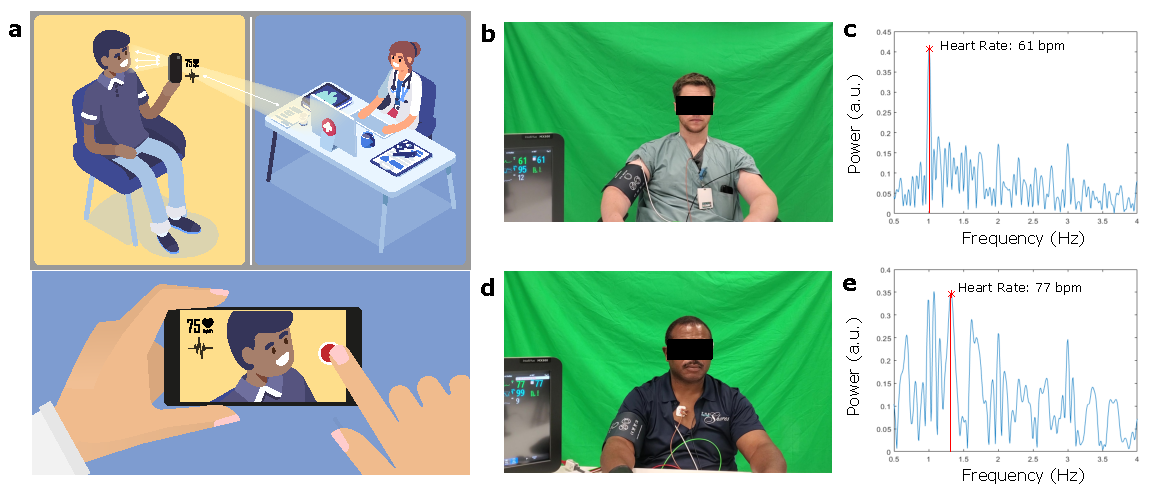
\includegraphics[width=\linewidth]{include/intro-fig.pdf}
    \caption{\textbf{Translating contactless camera-based HR sensing for telemedicine will require mitigating biased performance against dark skin tones.} (a) Cartoon illustration depicting the telemedicine application for the proposed contactless camera-based HR estimation. Telemedicine video-conferencing applications can be integrated with a software toolkit to display patient pulsatile signal and HR. (b) Frame of light skin tone subject from video. (c) Power spectrum of estimated pulsatile signal from light skin tone subject. Distinct peak at correct HR is shown in red. (d) Frame of dark skin tone subject from video. (e) Power spectrum of estimated pulsatile signal from dark skin tone subject. Frequency peak corresponding to correct HR is surrounded by noisy peaks. Videos used originate from the VITAL dataset. The CHROM algorithm with facial aggregation is employed to estimate the pulsatile signal. Credits: Illustration by Shelly Recchio.}
    \label{fig:teaser}
\end{figure}

Heart rate (HR) is an important clinical vital sign used in the evaluation of cardiorespiratory and hemodynamic stability. Conventional HR assessment is performed in-person at a clinic or hospital using specialized monitoring equipment. However, in recent years, healthcare delivery has progressed towards a remote model that uses telemedicine and mobile health (mHealth) technologies for patient evaluations. This transition has been accelerated by the COVID-19 pandemic \cite{annis_rapid_2020,ford_leveraging_2020,connolly_rapid_2020} in order to protect patients and healthcare workers from infectious exposure in a pandemic setting. The assessment of HR in patients with suspected COVID-19 is particularly important as COVID-19 has been associated with pre-existing cardiovascular disease \cite{nishiga_covid-19_2020}. Given the clinical relevance of HR in triage decisions, diagnosis, prognosis, and as a criterion for transfer to higher-level medical care, there is a pressing need to develop HR sensing solutions that can facilitate the rapidly growing domain of telemedicine-based care and remote patient monitoring.

Presently, HR sensing solutions for telemedicine and remote patient monitoring have relied on the adoption of wearable sensors to make plethysmographic or electrocardiographic measurements \cite{dinh-le_wearable_2019,lukas_emerging_2020}. Although such wearable technologies have seen major advances in the past decade \cite{kumar_mobile_2013, steinhubl_emerging_2015}, they still require large expenditure on production and distribution of hardware. This expense can create a barrier to adoption of mHealth technologies that disproportionately affects rural and socioeconomically burdened communities \cite{sawyer_wearable_2020}. 

In contrast to wearable sensors, recent methods have proposed using camera-based hardware present on modern-day smartphones in combination with signal processing and computer vision algorithms to estimate key vital signs, including HR \cite{li_current_2019}. Given the high penetration of mobile phone technology globally \cite{pew_demographics_2019}, such a solution would potentially have zero marginal cost, thereby offering clinicians a highly accessible and inexpensive method of assessing vital signs remotely. 

Camera-based HR sensing methods can be categorized into two distinct methodologies: contact-based and contactless. Contact-based methods, where the finger is typically placed on top the camera module, have already seen widespread applications in major smartphones \cite{proesmans_mobile_2019,li_current_2019}. Such methods show good performance, however, their utility for telemedicine video-conferencing visits is potentially limited as the camera module is covered during measurement. This prevents continuous monitoring of patient HR, visual well-being, and collection of other vitals such as respiratory rate and spatial blood perfusion maps. Contactless methods circumvent this limitation by remotely extracting a blood volume pulse (BVP) signal and corresponding HR estimate traditionally from facial videos \cite{rouast_remote_2018}. The consequence of capturing a larger field-of-view is a much weaker signal, and therefore worse performance. 

Remote photoplethysmography (R-PPG) is by far the most prominent technique used in literature for contactless camera-based HR sensing. R-PPG operates by looking for subtle color variations visible on the surface of human skin, caused by sub-dermal light absorption fluctuations from changes in blood volume and content. Early work conducted by Verkruysse \textit{et al.} \cite{verkruysse_remote_2008} showed that plethysmographic signals could be measured using ambient light and a consumer-grade digital camera. In order to accurately isolate and extract the correct BVP signal corresponding to the HR, several R-PPG algorithms have been proposed, including blind source separation (BSS)~\cite{poh_noncontact_2010,tsouri_constrained_2012,lewandowska_measuring_2011}, model-based~\cite{haan_robust_2013,wang_algorithmic_2017,song_new_2020,de_haan_improved_2014}, unsupervised data-driven~\cite{wang_novel_2016,tulyakov_self-adaptive_2016}, and supervised deep learning~\cite{chen_deepphys_2018,niu_rhythmnet_2020,yu_remote_2019,yu_remote_2019-1,nowara_benefit_2020,spetlik_visual_2018} methods. Unfortunately, the performance of existing R-PPG algorithms fluctuates with changes in illumination condition \cite{li_remote_2014}, subject motion \cite{mocco_motion_2016,de_haan_improved_2014,wang_exploiting_2015}, and skin tone \cite{nowara_meta-analysis_2020}. Moreover, assessment of these algorithms has typically been done on computer vision datasets that are not focused on telemedicine applications. Consequently, these datasets do not represent characteristics that are important for clinical translation such as a large population with diverse skin tone and gender representation and video data collection on end-user devices such as smartphones. 

The focus of this thesis is on developing a contactless camera-based HR sensing method for smartphone deployment that can successfully translate to telemedicine application. In particular, this thesis specifically addresses the bias for skin tone present in R-PPG algorithms. We provide a theoretical framework to understand the unique physics that underlies the inconsistency in R-PPG measurement across skin tones. From this, we establish that the bias is due to imaging noise, and appropriately propose R-PPG denoising methods to alleviate performance losses, including a novel algorithm that achieves overall state-of-the-art performance and large performance gains for dark skin tones. To assess the performance of the proposed method, we collect the first remote vital signs detection dataset focused on telemedicine applications that is demographically diverse. 

\section{Contributions}

In context of prior R-PPG related works, this thesis demonstrates the following technical contributions:

\begin{enumerate}
    \item A light-transport theory for R-PPG application that provides novel mathematical insights of R-PPG performance and biases with respect to skin tone.
    \item The first clinical telemedicine-focused remote vital signs dataset, named VITAL, that contains a diverse population of subjects under a variety of recording conditions. 
    \item A novel R-PPG algorithm that achieves overall state-of-the-art performance and large performance gains for dark skin tones on the VITAL dataset.
\end{enumerate}

% \section{Organization}


  
%
% theory.tex
% Copyright (C) 2021 by Krish Kabra, <krish@kabra.com>.
%

\chapter{Theory} \label{chap:theory}

\section{Origins of Skin Tone Bias in R-PPG}

\begin{figure}[t]
    \centering
    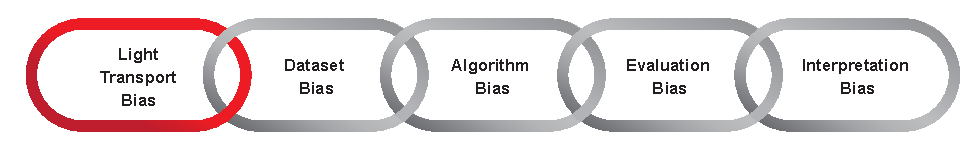
\includegraphics[width=\linewidth]{include/F_chain2.pdf}
    \caption{\textbf{The chain of biases in vision.} At the top of the chain lies the decision-making biases, which includes interpretation bias caused by the inappropriate analysis of results and evaluation bias caused by inappropriate benchmarks and statistical analyses used for evaluation. In the middle of the chain lies the computational biases, which includes algorithm bias caused by inappropriate machine-learned or software-embedded features and dataset bias caused by uneven distribution of training data. Finally, at the bottom of the chain lies the physical bias, which for vision systems is light transport bias caused by the physical laws and principles of sensing equipment. The focus of this section is highlighting the light transport bias in R-PPG.}
    \label{fig:chain_bias}
\end{figure}

\begin{figure}
    \centering
    \includegraphics[width=\linewidth]{include/fig-light-transport-skin.pdf}
    \caption{\textbf{Skin melanin fraction plays an important role when assessing physiological properties from human skin.} (a) The world map of skin tone of indigenous people shows skin coloration is strongly correlated with UV radiation levels. This suggests melanin pigementation, which determines skin tone, has a part in regulating the effects of radiation on the contents of blood vessels located in the dermis. (b) A two-layer skin model based on prior biorealistic rendering works is used to develop the light transport theory for R-PPG. The incident light ray attenuates through the epidermis. Following dermal reflection and another epidermal attenuation, the resultant ray properties are dependent on human physiological quantities. Source: Map is adapted from Jablonski \& Chaplin (2000).}
    \label{fig:light_transport_skin}
\end{figure}

In recent years, there has been a rising concern regarding the bias of vision-based systems \cite{brandao_age_2019,buolamwini_gender_2018,klare_face_2012,vangara_characterizing_2019}. A biased system or device is one that operates in a manner that disadvantages certain demographic groups and influences inequity. The important work of Nowara \textit{et al.} \cite{nowara_meta-analysis_2020} highlights the bias encompassing R-PPG technologies with respect to subject skin tone and gender, namely the poor performance for dark skin tones and women. To address this complex issue of bias, the computer vision community has rightly pointed out factors that include dataset bias, algorithmic bias, and decision-making bias. However, there is another type of bias that is less discussed: the bias encountered by the laws of physics. Vision-based systems, including R-PPG, rely on light-sensing cameras; however, the physics of light itself may involve bias. 

Kadambi \cite{kadambi_achieving_2021} highlights the various biases that may exist in medical devices, namely physical bias, computational bias, and interpretation bias. Figure~\ref{fig:chain_bias} extends this idea and outlines the chain of biases in vision-based systems. At the top of the chain lies the decision-making biases, which includes interpretation bias caused by the inappropriate analysis of results and evaluation bias caused by inappropriate benchmarks and statistical analyses used for evaluation. In the middle of the chain lies the computational biases, which includes algorithm bias caused by inappropriate machine-learned or software-embedded features and dataset bias caused by uneven distribution of training data. Finally, at the bottom of the chain lies the physical bias, which for vision systems is light transport bias caused by the physical laws and principles of sensing equipment. 

Light transport bias for medical devices is a rarely considered factor. Traditionally, medical devices rely on empirically determined calibration constants to estimate physiological parameters. In the case of pulse oximeters, the constants used do not account for variations in skin structure, including skin melanin fraction. However, Jablonski \& Chaplin \cite{jablonski_evolution_2000} concluded that one of the main roles of melanin pigmentation is the regulation of the effects of UV radiation on the contents of blood vessels located in the dermis. This conclusion was made after observing a high correlation between the skin tone of indigenous people around the world with absolute latitude and UV radiation, visually seen in Figure~\ref{fig:light_transport_skin}a. Therefore, by not accounting for the role of melanin or skin tone, pulse oximeters fail to calibrate for a key variable that affects skin light absorption and, consequently, blood oxygenation estimation. This fact has come to light recently with works highlighting the skin tone bias present in pulse oximeters \cite{sjoding_racial_2020}. 

In the following section, we establish a novel light transport theory for R-PPG that enables valuable insight into the origins of the skin tone bias. We will show that the signal strength reduces with increasing skin melanin content for all color channels, as intuitively expected. The decreasing signal strength leads us to an analysis of imaging noise, which is the major noise phenomenon at play in this case. Knowledge that the root of bias in R-PPG is due to light transport bias, which is exacerbated by imaging noise, leads us to a novel R-PPG algorithm described in Chapter~\ref{chap:methods} that significantly reduces the skin tone bias without fundamental changes to the hardware of the system. Beyond the light transport bias, this thesis also utilizes a new telemedicine-focused dataset that alleviates dataset bias, and highlights how previous R-PPG algorithms exhibit algorithmic bias. 

\section{Light Transport for R-PPG}

% \begin{figure}[t]
%     \centering
%     \includegraphics[height=3in]{include/fig_skin.pdf}
%     \caption{\textbf{A two-layer skin model used in prior biorealistic rendering works is used to develop the light transport theory for R-PPG.} The incident light ray attenuates through the epidermis. Following dermal reflection and another epidermal attenuation, the resultant ray properties are dependent on human physiological quantities.}
%     \label{fig:skin_model}
% \end{figure}

Plethysmographic estimation methods are enabled through the sensing of blood perfusion in the face. Specifically, the presence of varying volumes of blood under the skin manifest as minute changes in reflection properties of the overall skin system, as viewed by a camera. It is by identifying these changes that relevant physiological properties may be estimated. 

In order to set up a novel light transport theory for R-PPG, we utilize existing biorealistic graphical rendering models~\cite{krishnaswamy_biophysically_2004,igarashi_appearance_2007} and extend them for R-PPG signal generation. Figure~\ref{fig:light_transport_skin}b shows the skin model assumed for our computations, similar to~\cite{alotaibi_biophysical_2017}. Specifically, a two layer skin model is assumed. The incident light undergoes attenuation while passing through the epidermis, while it undergoes scattering driven reflection at the dermis. 

% \subsection{Epidermal Transmission}
We start with describing the epidermal transmission. Following the Beer-Lambert Law, 
\begin{equation} \label{eqn:T_epidermis}
    \mathbf{T_{epi}(\boldsymbol{\lambda})=e^{-\boldsymbol\mu_{a,epi}(\boldsymbol\lambda)}},
\end{equation}
Where $\mathbf{\boldsymbol\mu_{a,epi}(\boldsymbol\lambda)}$ is the absorption coefficient of the epidermis. Typically, this is modelled as a convex combination of skin tissue and melanin absorption,
\begin{equation} \label{eqn:mu_epidermis}
    \mathbf{\boldsymbol\mu_{a,epi}(\boldsymbol\lambda)=f_{mel}\boldsymbol\mu_{a,mel}(\boldsymbol\lambda)+(1-f_{mel})\boldsymbol\mu_{a,ski}(\boldsymbol\lambda)}.
\end{equation}

$\mathbf{\boldsymbol\mu_{a,ski}(\boldsymbol\lambda)}$, the skin tissue absorption coefficient, is a biological parameters which is known. $\mathbf{\boldsymbol\mu_{a,mel}(\boldsymbol\lambda)}$ may be defined as,
\begin{equation} \label{eqn:mu_melanin}
    \mathbf{\boldsymbol\mu_{a,mel}(\boldsymbol\lambda)=f_{eum}\boldsymbol\mu_{a,eum}(\boldsymbol\lambda)+(1-f_{eum})\boldsymbol\mu_{a,phm}(\boldsymbol\lambda)},
\end{equation}
Where ${\mathbf{\boldsymbol\mu_{a,eum}(\boldsymbol\lambda)}}$ is the absorption coefficient of eumelanin and $\mathbf{\boldsymbol\mu_{a,phm}(\boldsymbol\lambda)}$ is the absorption coefficient of pheomelanin, all biophysical known parameters. By combining Equations~\ref{eqn:T_epidermis}, \ref{eqn:mu_epidermis} and \ref{eqn:mu_melanin}, the epidermal transmission may be accurately modelled.

% \subsection{Dermal Reflection} 
We move towards describing the dermal reflection. This model follows the Kubelka-Munk theory for scattering-dependent reflection. Specifically, the fraction of reflected light, as a function of wavelength, is given by,
\begin{equation}
    \mathbf{R_{d}(\boldsymbol\lambda)=\frac{(1-\boldsymbol\beta(\boldsymbol\lambda))^2(e^{K(\boldsymbol\lambda)d_{der}}-e^{-K(\boldsymbol\lambda)d_{der}})}{(1+\boldsymbol\beta(\boldsymbol\lambda))^2e^{K(\boldsymbol\lambda)d_{der}}-(1-\boldsymbol\beta(\boldsymbol\lambda))^2e^{-K(\boldsymbol\lambda)d_{der}}}}
\end{equation}
Here, $\mathbf{\boldsymbol\beta(\boldsymbol\lambda)}$ and $\mathbf{K(\boldsymbol\lambda)}$ are deterministically related to $\mathbf{\boldsymbol\mu_{a,der}(\boldsymbol\lambda)}$ (dermal absorption coefficient) and $\mathbf{\boldsymbol\mu_{s,der}(\boldsymbol\lambda)}$ (reduced dermal scattering coefficient, known~\cite{anderson_optics_1981}). Similar to previously, the dermal absorption coefficient and the blood absorption coefficient are understood as convex combinations shown below:
\begin{equation}
    \mathbf{\boldsymbol\mu_{a,der}(\boldsymbol\lambda)=f_{bld}\boldsymbol\mu_{a,bld}(\boldsymbol\lambda)+(1-f_{bld})\boldsymbol\mu_{a,ski}(\boldsymbol\lambda)}
\end{equation}
\begin{equation}
    \mathbf{\boldsymbol\mu_{a,bld}(\boldsymbol\lambda)=f_{oxy}\boldsymbol\mu_{oxy}(\boldsymbol\lambda)+(1-f_{oxy})\boldsymbol\mu_{dox}(\boldsymbol\lambda)}
\end{equation}
Here, various factors include blood reflection, skin baseline reflection, oxygenated blood reflection and deoxygenated blood reflection respectively.

% \subsection{Overall Reflection} 
Given the expressions for epidermal transmission and dermal reflection, the expression for overall reflection is given by,
\begin{equation}
    \mathbf{R(\boldsymbol\lambda) = T{^2}_{epi}.R_{d}(\boldsymbol\lambda)}.
\end{equation}

Then, the overall intensity captured in channel $\mathbf{c}$ of the camera is given by,
\begin{equation}
    \mathbf{I_c=\boldsymbol\int_{\boldsymbol\lambda}E(\boldsymbol\lambda)S_{c}(\boldsymbol\lambda)R(\boldsymbol\lambda)d\boldsymbol\lambda},
\end{equation}
Where $\mathbf{E(\boldsymbol\lambda)}$ is the source spectral distribution and $\mathbf{S_{c}(\boldsymbol\lambda)}$ is the camera spectral response for channel $\mathbf{c}$.

\section{R-PPG Signal Strength} 

The R-PPG signal arises out of a variation in the blood volume fraction, $\mathbf{f_{bl}}$ under the skin. Our interest is in the signal strength across camera channels, $\boldsymbol\Sigma_{c}$, which can be defined as \textit{the maximum variation in the captured intensity}. Mathematically,
\begin{equation}
\begin{split}
    &\mathbf{\boldsymbol\Sigma_{c}=\boldsymbol\Delta I_c\boldsymbol\approx \Big|\frac{\boldsymbol\partial I_c}{\boldsymbol\partial f_{bl}}\Big|\cdot\boldsymbol\Delta f_{bl}}
\end{split}
\end{equation}
Since $\mathbf{R(\boldsymbol\lambda)}$ is the only term dependent on $\mathbf{f_{bl}}$,
\begin{equation}
\begin{split}
    &\mathbf{\boldsymbol\Sigma_{c}\boldsymbol\approx  \Big|\boldsymbol\int_{\boldsymbol\lambda}E(\boldsymbol\lambda)S_{c}(\boldsymbol\lambda)\frac{\boldsymbol\partial R}{\boldsymbol\partial f_{bl}}\Bigg|_{\overline{f_{bl}}} d\boldsymbol\lambda \Big| \cdot \boldsymbol\Delta f_{bl}},
\end{split}
\end{equation}
Where $\mathbf{\overline{f_{bl}}}$ is the average blood volume fraction, typically around $0.05$. This approximation holds true since $\mathbf{f_{bl}}$ only varies by a small amount, typically around $0.05$. 

This plethysmographic signal rides on top of the average skin tone color, given by
\begin{equation}
    \mathbf{\boldsymbol\Gamma_c=\boldsymbol\int_{\boldsymbol\lambda}E(\boldsymbol\lambda)S_{c}(\boldsymbol\lambda)R(\boldsymbol\lambda)\Big|_{\overline{f_{bl}}} d\boldsymbol\lambda}.
\end{equation}

Since, $\boldsymbol\Sigma_{c}$ and $\boldsymbol\Gamma_{c}$ are both dependent on $\mathbf{f_{mel}}$, as a result of the dependence of $\mathbf{R(\cdot)}$ on the same, we refer to these as $\mathbf{\boldsymbol\Sigma(f_{mel})}$ and $\mathbf{\boldsymbol\Gamma(f_{mel})}$ subsequently.

% {\color{red} 
% \begin{enumerate}
%     \item Add parameter values used/the source paper for the same, for reproducability.
%     \item Not clear what you mean by average camera response function. Also, where did we get the average response function from? We should cite our sources for reproducability. Same goes for light source characteristics.
% \end{enumerate}
% }

\begin{figure}[t]
    \centering
    \includegraphics[width=\linewidth]{include/fig_strength_dB.pdf}
    \caption{\textbf{The R-PPG signal strength is critically related to skin melanin fraction as well as scene lighting.} As opposed to previously accepted fact, the three channels may contain differing amounts of signal information, depending on regime of operation.}
    \label{fig:signal_strength}
\end{figure}

Figure~\ref{fig:signal_strength} shows the signal strength plots for the three camera color channels, across lighting conditions. We use average camera response functions $\mathbf{S_c(\boldsymbol\lambda)}$ to identify responsiveness of each of the channels to incident light. We also generate signal strength across common light source characteristics. These plots provide incisive detail: the overall signal strength decays with increasing skin melanin fraction. Additionally, while previous works~\cite{verkruysse_remote_2008,haan_robust_2013,wang_algorithmic_2017} have empirically determined that the green channel holds maximum R-PPG signal information, we show for the first time that this in-fact heavily depends on melanin fraction and scene lighting. While the green channel is dominant for light skin tones, for darker skin tones, the channel-wise signal strength depends significantly on lighting conditions and skin tone.

\section{Effect of Imaging Noise on R-PPG}\label{sec:effect_noise_RPPG}

The goal of this subsection is to understand the relationship between imaging noise and R-PPG algorithm estimation. Imaging noise refers to the inherent noise that arises due to the image capture process in a commercial camera. This arises due to various effects related to photon arrival processes, thermal noise in electronics and the quantization noise associated with digitally capturing images \cite{hasinoff_noise-optimal_2010}. For
pixels below the saturation level, the noise can be modelled as follows: 
\begin{equation} \label{eqn:imaging_noise_model}
    \sigma_{pixel}^2 = \frac{\Phi t}{g^2} + \frac{\sigma_{r}^2}{g^2} + \sigma_{q}^2
\end{equation}
where $\Phi$ is the radiant power of light collect, $t$ is the exposure time, $g$ is the sensor gain (a constant for a given image), and $\sigma_r$ and $\sigma_q$ are camera noie parameters (also constant). 

Using this noise model, we can the estimate the entire R-PPG signal to noise ratio (SNR) for a pixel of a particular intensity and color channel $c$ as follows:
\begin{equation} \label{eqn:SNR_rPPG}
    \mathbf{SNR_c} = \frac{\mathbf{\boldsymbol\Sigma_{c}}t}{\sqrt{\frac{\mathbf{\boldsymbol\Gamma_{c}}t}{g^2} + \frac{\sigma_{r}^2}{g^2} + \sigma_{q}^2}}
\end{equation}
Here, we assume that the radiant power of light collected $\Phi$ is equal to the average skin tone color. 

\begin{figure}[t]
    \centering
    \includegraphics[width=\linewidth]{include/fig_SNR_dB.pdf}
    \caption{\textbf{The R-PPG SNR drastically worsens with increasing skin melanin fraction.} As expected, the R-PPG SNR reduces by orders of magnitude as the skin melanin fraction increases. Therefore, mitigating the skin tone bias present in R-PPG will require strategies that emphasize capturing more signal and reducing noise.}
    \label{fig:SNR_theory}
\end{figure}

Figure~\ref{fig:SNR_theory} shows the R-PPG SNR plots for the three camera color channels, across lighting conditions. These observations are similar to those of the R-PPG signal strength, namely that the SNR decays with increasing skin melanin fraction. This leads us to the following inferences: 
\begin{enumerate}[label=(\roman*)]
    \item \textbf{Imaging noise creates skin tone bias (and lighting bias):} The performance gap across skin tones, as well as across lighting differences, can be understood in terms of imaging noise. Darker skin regions have lower signal strength that manifest as lower pixel value changes in the video. This results in poorer SNRs. Note that this inference also holds true for shadowed regions, thereby extending this analysis towards understanding lighting bias.
    \item \textbf{Imaging noise and specular reflections degrade the R-PPG signal:} Imaging noise, coupled with specular highlights due to lighting, are the major contributing factors to signal degradation. The corruption due to imaging noise depends on signal intensity. The corruption due to specular highlights depends on lighting conditions- regions with strong specular highlights have relatively lower PPG signal information. Combating the highlighted biases in existing R-PPG would therefore involve a principled approach towards reduction of the above highlighted imaging noise and specular highlight removal. Note that specular highlight removal, in addition to reducing lighting related biases, also indirectly affects skin tone bias: darker skin subjects are worse affected by these interferences, since the intensity difference between the signal and the highlight is much more. 
\end{enumerate}

We conclude that addressing this low-level light transport bias must occur in order to drastically mitigate the skin tone bias present in R-PPG. Biases higher up the chain of biases, such as algorithmic or dataset bias, must also be addressed, but may not necessarily overcome this fundamental physics-based problem. Therefore, image and signal processing strategies to increase signal capture and reduce noise may drastically improve performance for darker skin tone subjects as opposed to modifications to signal inference algorithms. With the inferences from this chapter in mind, we motivate our novel R-PPG algorithm outlined in the following Methods section.

  
%
% methods.tex
% Copyright (C) 2021 by Krish Kabra, <krish@kabra.com>.
%

\chapter{Methods} \label{chap:methods}

\section{VITAL Dataset}

\begin{figure}
    \centering
    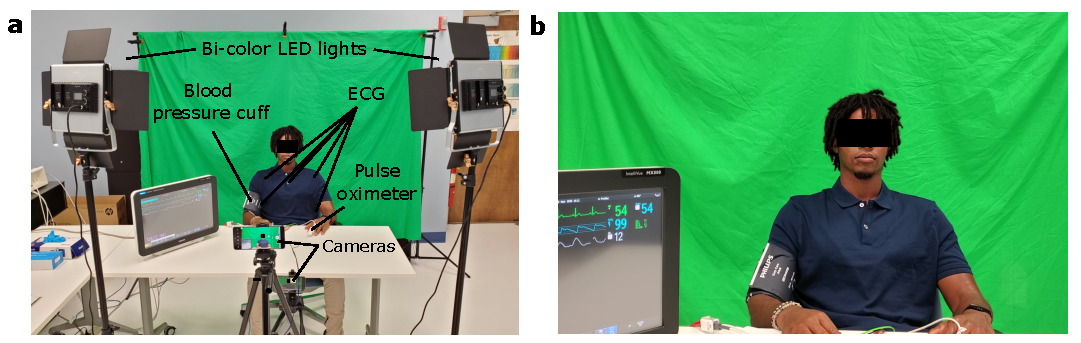
\includegraphics[width=\linewidth]{include/exp_setup_v2.pdf}
    \caption{\textbf{Constructing a diverse remote vital sign monitoring dataset with a focus on telemedicine applications.} (a) Experimental setup employed during the construction of the VITAL dataset. Two bi-color LEDs are used for controlled illumination of the subject, and laboratory tube LEDs are used for ambient illumination. The Philips IntelliVue MX800 patient monitor is utilized for ground truth vital sign monitoring. The subject wears a blood pressure cuff, 5-ECG leads, and a finger pulse oximeter, which is connected to the MX800 unit. Two smartphone cameras at differing viewing angles capture video of the subject. (b) Example frame from video captured by the front smartphone camera. Written consent was obtained from the subject for using their image in the publication.}
    \label{fig:exp_setup}
\end{figure}

To validate the performance of camera-based vital sign detectors, we construct the Vital-sign Imaging for Telemedicine AppLications (VITAL) dataset. The focus of this dataset is to represent diversity in factors that are relevant to telemedicine setups, including: (i) smartphone deployment, (ii) camera view angle, (iii) recording condition (lighting variation and talking), and (iv) patient demographic diversity. We address each of these aspects individually:

\begin{enumerate}[label=(\roman*)]
    \item \textbf{Smartphone deployment:} The ubiquity of smartphones globally has led to the development of patient portals, many of which can be accessed via smartphone applications that can be downloaded by patients \cite{mosa_systematic_2012,ventola_mobile_2014,boulos_how_2011}. Such applications have been used for hosting telemedicine appointments. A deployable remote HR estimation solution with a focus on telemedicine must be able to work efficiently on smartphone cameras by considering factors including video compression \cite{yu_remote_2019,nowara_systematic_2021,nowara_combating_2019} and algorithmic complexity. Moreover, the solution must achieve success independent of camera type. Hence, the VITAL dataset uses different smartphone cameras for each view angle. The use of more than one smartphone imager inspires the development of algorithms that can scale to a variety of device-agnostic telemedicine conditions. 
    \item \textbf{Camera view angle:} In a telemedicine setting, there can also be a variety of camera angles that the algorithm must work on. In order to facilitate this verification, the VITAL dataset consists of two camera view angles for all the videos of each subject (as seen in Figure~\ref{fig:exp_setup}).
    \item \textbf{Recording condition:} Another essential factor involves testing algorithms across a range of recording conditions, to promote the development of algorithms that can operate in the “wild”. The dataset consists of four recording conditions: (1) controlled lighting at 5600K (“cool” lighting) with the subject remaining stationary, (2) controlled lighting at 3200K (“warm” lighting) with the subject remaining stationary, (3) ambient room lighting- distributed white lighting- with the subject remaining stationary, and (4) ambient room lighting with the subject speaking. Additionally, a green screen backdrop is kept to potentially enable digital modification of background scenery.
    \item \textbf{Patient demographic diversity:} The VITAL dataset consists of 59 subjects spread across skin tone, age, gender, race, and ethnic backgrounds. Subject characteristics (gender, age, height, weight, body mass index, race, and ethnicity) are summarized in Table~\ref{tab:demographic} using mean (SD), median (IQR), or frequency (\%), unless otherwise noted. For the purpose of this study, we split the subjects into three skin tone categories based on the Fitzpatrick (FP) skin type scale \cite{fitzpatrick_validity_1988}: light, consisting of skin tones in the FP 1 and 2 scales, medium, consisting of skin tones in the FP 3 and 4 scales, and dark, consisting of skin tones in the FP 5 and 6 scales. This aggregation allows for more relevant trends, since any two consecutive FP scale categories are reasonably close.
\end{enumerate}

\begin{table}[]
\begin{center}
\scalebox{0.83}{
\begin{tabular}{lcl}
Total number of participants in study & \multicolumn{2}{c}{59} \\
 & \multicolumn{1}{l}{} &  \\
\textbf{Physical Demographics} & \multicolumn{1}{l}{\textbf{Mean}} & \textbf{Median} \\ \hline
Age (years) & 34 (10) & \multicolumn{1}{c}{34 (26-40)} \\
Height (cm) & 172 (10) & \multicolumn{1}{c}{174 (164-180)} \\
Weight (kg) & 73 (19) & \multicolumn{1}{c}{71 (57-82)} \\
Body Mass Index (kg m$^{-2}$) & 24 (7) & \multicolumn{1}{c}{24 (21-25)} \\
 & \multicolumn{1}{l}{} &  \\
\textbf{Sex} & \multicolumn{2}{l}{\textbf{\# of participants}} \\ \hline
Male & \multicolumn{2}{c}{36 (61\%)} \\
Female & \multicolumn{2}{c}{23 (39\%)} \\
 & \multicolumn{1}{l}{} &  \\
\textbf{Race} & \multicolumn{2}{l}{\textbf{\# of participants}} \\ \hline
White & \multicolumn{2}{c}{29 (49\%)} \\
Asian & \multicolumn{2}{c}{18 (31\%)} \\
Black or African American & \multicolumn{2}{c}{9 (15\%)} \\
Native Hawaiian or other Pacific Islander & \multicolumn{2}{c}{0 (0\%)} \\
American Indian or Alaska Native & \multicolumn{2}{c}{2 (3\%)} \\
Unknown & \multicolumn{2}{c}{1 (2\%)} \\
 & \multicolumn{1}{l}{} &  \\
\textbf{Ethnicity} & \multicolumn{2}{l}{\textbf{\# of participants}} \\ \hline
Hispanic/Latino & \multicolumn{2}{c}{7 (12\%)} \\
non-Hispanic/Latino & \multicolumn{2}{c}{52 (88\%)} \\
 & \multicolumn{1}{l}{} &  \\
\textbf{Skin Type} & \multicolumn{2}{l}{\textbf{\# of participants}} \\ \hline
Light & \multicolumn{2}{c}{21 (36\%)} \\
Medium & \multicolumn{2}{c}{26 (44\%)} \\
Dark & \multicolumn{2}{c}{12 (20\%)}
\end{tabular}} 
\end{center}

\caption{\textbf{Demographic characteristics of volunteers in the VITAL dataset.} Subject characteristics (gender, age, height, weight, body mass index, race, and ethnicity) are summarized using mean (SD), median (IQR), or frequency (\%).}
\label{tab:demographic}
\end{table}

The human study protocol was approved by the UCLA Institutional Review Board (IRB\#20-001025-AM-00001), and participants provided written informed consent to take part in the study. Figure~\ref{fig:exp_setup} shows the data collection setup. Each subject is made to sit on a height-adjustable chair, in the field of view of two cell-phone cameras (with different view angles): one camera (Samsung Galaxy S10) is perfectly front-on, while the other (Samsung Galaxy A51) is directly in front of the face, at a dip (lower) of 15 degrees. The front-on camera is placed approximately 130 cm from the subject, and the lower camera at a dip is approximately 90 cm from the subject. The height of the chair is chosen so that the subject is centered in the front-on frame. The controlled lights are set up on either side of the front-on camera, with a baseline of 100 centimeters between them.

As aforementioned, we record subjects using these cameras under four different scene conditions: (1) controlled lighting at 5600K (“cool” lighting) with the subject remaining stationary, (2) controlled lighting at 3200K (“warm” lighting) with the subject remaining stationary, (3) ambient room lighting (distributed white LED lighting) with the subject remaining stationary, and (4) ambient room lighting with the subject speaking. Controlled lighting is enabled by a pair of professional bi-color LED photography lights (Neewer Bi-Color 480 LED). The controlled lighting recording conditions were enabled with the room lights off, allowing for fine-tuned control over the illumination spectral properties. As incorporating controlled lighting only enables a front-facing illumination angle, two recording conditions in ambient room lighting were captured where the subject was lit more completely from several angles. The final recording condition involved variations in the subject, including talking, natural head movements, and facial expressions. Each scene recording session lasts for 2 minutes, for a total of 16 minutes of video footage across 8 videos. 

During data collection, volunteers are fitted with standard anesthesiology cardiopulmonary monitors: pulse oximeter (Red DCI, Masimo), blood pressure cuff (Comfort Care, Philips), and 5-lead electrocardiogram (Philips IntelliVue). To collect vital sign data, we utilize the Philips IntelliVue MX800 patient monitor to perform real time monitoring of four vital signs- HR, respiratory rate, oxygen saturation, and non-invasive continuous blood pressure- of which three waveforms are collected (ECG, PPG and respiration). We use the open source tool VSCapture \cite{karippacheril_data_2013} to collect data onto a computer using the MX800’s local area network communication protocol. The MX800’s estimated numeric values for the vital signs are sampled every 1 second, while the waveforms are sampled at variable frequencies. The ECG signal is sampled between 400-600 Hz, the PPG signal between 100-150Hz and the respiration between 40-60Hz.  Continuous non-invasive blood pressure estimates occur when the blood pressure cuff is activated, which is approximately once every 30 seconds. 

A total of 60 subjects participated in the study. Due to data collection errors, 1 subject is excluded from the experiment. Therefore, the final VITAL dataset consists of 472 videos ($\sim$944 minutes) of 59 subjects and their vital signs. The demographic characteristics of these volunteers is given in Table~\ref{tab:demographic}.

\section{The Diverse R-PPG pipeline}

\begin{figure}
    \centering
    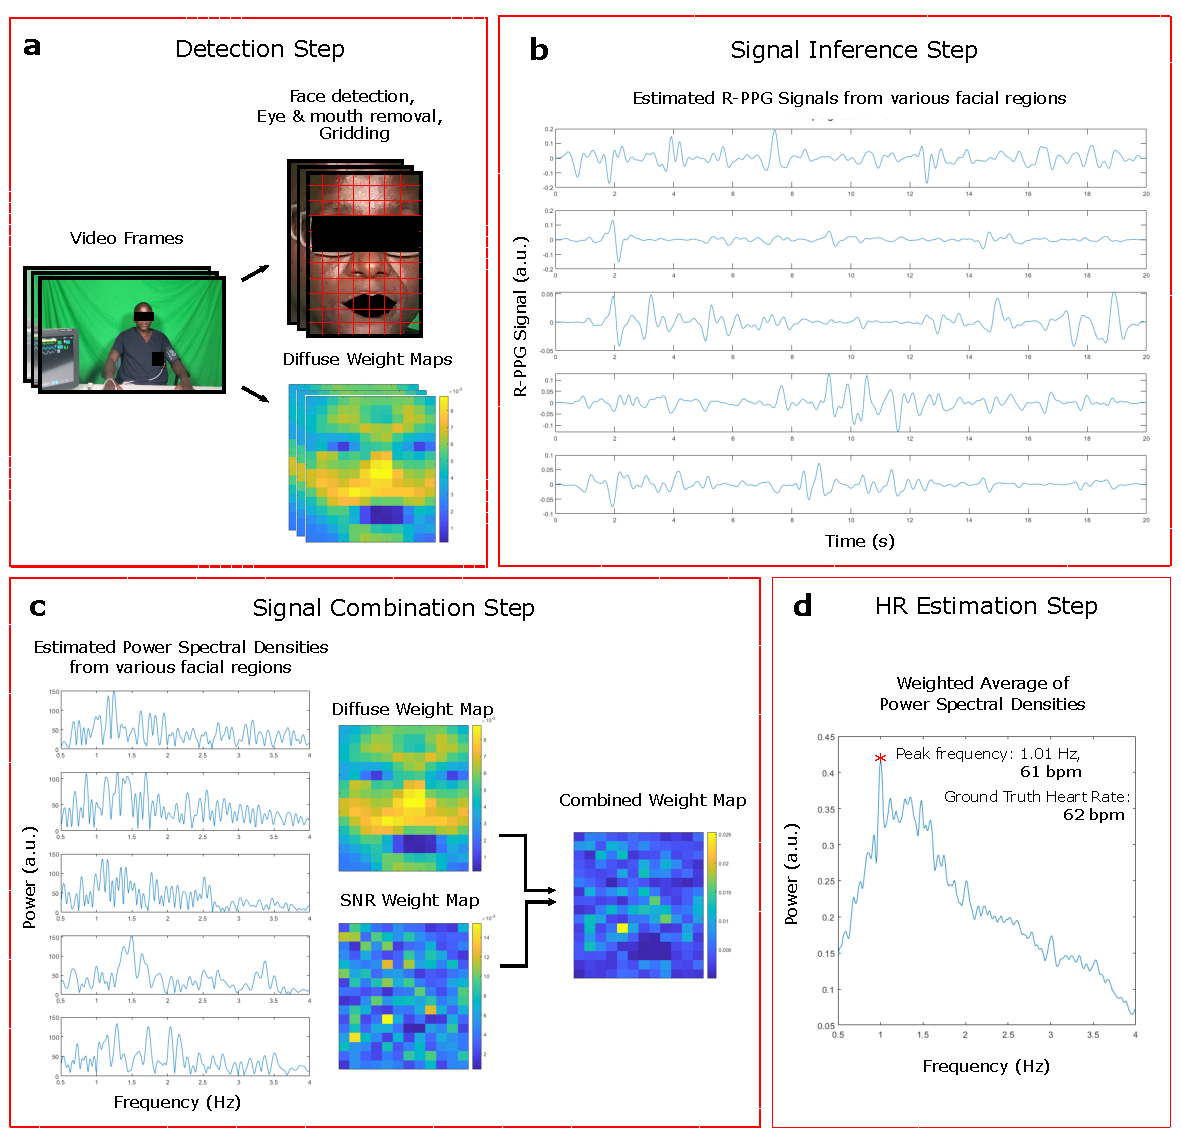
\includegraphics[width=0.75\linewidth]{include/fig6-pipeline.pdf}
    \caption{\textbf{The proposed contactless camera-based heart rate estimation algorithm consists of 4 steps.} The proposed novelty in the signal combination step of the pipeline incorporates skin diffuse information weighting, in addition to SNR weighting, to fuse signal information in the frequency-domain space in order to achieve robust R-PPG performance across skin tones. Written consent was obtained from the subject for using their image in the publication.}
    \label{fig:pipeline}
\end{figure}

There are four components to a typical R-PPG pipeline: (a) detection, which identifies facial regions of interest (ROI) in the video frame, (b) signal inference, which uses the RGB time series signals to estimate the pulsatile waveforms from the ROIs, (c) signal combination, which combines the information from the various estimated pulsatile waveforms, and (d) HR estimation, which estimates the HR from the combined information. 

From Section \ref{chap:theory}, we concluded that on top of other skin tone biases present in R-PPG algorithms and datasets, the main contributing factor to R-PPG skin tone bias is the fundamental light-transport bias that exists for subjects with a higher skin melanin fraction. Specifically, we showed that the R-PPG SNR drastically worsens with increasing skin melanin fraction, and therefore mitigating the skin tone bias present in R-PPG will require strategies that emphasize capturing more signal and reducing noise. As such, the primary innovation to the typical R-PPG pipeline will be in the signal combination step.  

The Diverse R-PPG pipeline is visually described in Figure~\ref{fig:pipeline}. The video is first passed through a neural network-based face detector \cite{zhang_joint_2016}, in order to identify the face region in the frame. Using feature point detectors \cite{kazemi_one_2014}, the eye and mouth regions are identified and explicitly removed from the videos (since these regions do not contribute to the pulsatile signal). Additionally, the diffuse component of the face is estimated using a specular highlight removal algorithm \cite{yang_real-time_2010}. Regions of interest are then obtained by dividing the facial frames into 192 grids of equal height and width. This is the detection step. The next steps, namely signal inference and signal combination and HR estimation, are carried out for smaller video-windows of 20 seconds length with an overlap of 10 seconds.

For signal inference, we choose the CHROM \cite{haan_robust_2013} signal extraction method due to its versatility and open availability of code \cite{mcduff_iphys_2019}. The spatially averaged RGB time series from each grid is used to estimate a pulsatile waveform. This waveform is then filtered using a 5th-order Butterworth bandpass filter with pass-band frequencies of [0.7, 4] Hz. These waveforms are used in the following signal combination step. 

In order to capture more signal and reduce noise, the pulsatile waveforms from the various ROIs on the face must be combined in a sensible manner. Traditionally, this combination does not occur after signal inference, but rather before when the pixels from the face are averaged for each frame. This is equivalent to defining only one grid or ROI, which is all the (skin-)pixels on the face. However, this naive averaging may not be optimal for noise reduction-- for example, regions on the face not corresponding to skin or containing large amounts of motion will contain noisy pulsatile information. 

To improve upon this, previous approaches have sought to modify this averaging process using a weighted average scheme. Most commonly, approaches have used a measure such as SNR at peak frequency of the estimated pulsatile waveform to characterize the `goodness' of each signal \cite{haan_robust_2013,po_block-based_2018,li_model-based_2020,kumar_distanceppg_2015,bobbia_unsupervised_2019}, and therefore be used as weights. The SNR can be estimated for a signal $s(t)$ (frequency domain $S(f)$) given a frequency $p$ that we suspect corresponds to the HR as follows:

\begin{equation}
    SNR=\frac{\int_{p-w}^{p+w}{\left|S(f)\right|^2df}+\int_{2(p-w)}^{2(p+w)}{\left|S(f)\right|^2df}}{\int_{-\infty}^{\infty}{\left|S(f)\right|^2df}-\int_{p-w}^{p+w}{\left|S(f)\right|^2df}-\int_{2(p-w)}^{2(p+w)}{\left|S(f)\right|^2df}}
\end{equation}

where $w$ is the peak window size for estimation (for this work’s experiments, we use $w=0.1$Hz). This essentially defines the signal power to be contained within a narrow-band of the fundamental and first harmonic of the HR frequency $p$, and regards the remaining signal power as noise.  

There are two major drawbacks to this method of signal combination. First, this method relies heavily on a good estimate of the initial HR frequency $p$. The $p$ used typically corresponds to the peak frequency of the signal from the naive facial aggregation method. As R-PPG is fundamentally biased with respect to skin tone, the estimate for $p$ is typically worse for darker skin tones. Moreover, the effect of noise more greatly affects darker skin tones. Consequently, it is empirically observed that the SNR weights for dark skin tones is far more variable window-to-window and sparse spatially. This means that this SNR weighting method of signal combination can actually worsen the skin-tone bias present in R-PPG (we observe this in our Results section). Second, this method of signal combination is done in the time-domain. However, it is not guaranteed that the pulsatile waveforms from different ROIs are aligned in time, either due to physical separation between the regions or due to the rolling-shutter of the video-camera. In other words, there may be a phase delay between the signals. The rolling-shutter effect is particularly relvant for R-PPG using smartphone cameras as highlighted by Mironenko \textit{et al.} \cite{mironenko_remote_2020}. 

To combat these issues, Diverse R-PPG makes two major novelities to the signal combination step: 
\begin{enumerate}[label=(\roman*)]
    \item \textbf{Combination in frequency-domain:} Ultimately, the goal is to estimate the HR of the subject. This relies on the frequency information contained within the estimated pulsatile waveform. The phase delay between estimated signals from different ROIs only affects the frequency content by a scalar constant. Therefore, by performing signal combination in the frequency-domain, namely through averaging the power spectral densities (PSD) of the inferred signals, sensible signal combination can be done without introducing additional artifacts. 
    \item \textbf{Novel weighting scheme:} From Section~\ref{sec:effect_noise_RPPG}, we concluded that specular reflections degrade the R-PPG signal. From the detection step, the estimated diffuse component can therefore be used as additional weights. The SNR weights from previous works and the novel diffuse weights are multiplied together and renormalized to arrive at the final weights used to combine the signals. The diffuse weights play two key roles: first, they can remove specular affected regions from the average explicitly. Second, they combat the sparsity issue observed in traditional SNR weights, since the diffuse component is continuous and non-sparse. 
\end{enumerate}

After computing the weighted average PSD using the novel weights and individual PSDs from the gridded pulsatile signals, the final HR is estimated by simply choosing the peak frequency. This summarizes the Diverse R-PPG pipeline for a single window. The pipeline can be iterated over multiple overlapping windows to estimate a beat-to-beat HR.  

\section{Benchmark methods and techniques}

To benchmark the performance of the proposed method, we compare the proposed method against previous R-PPG algorithms similar to our method. We compare with the two most common categories of signal combination steps that were described in the previous section, namely the naive pixel averaging, which we refer to as facial aggregation (c.f. \cite{poh_noncontact_2010,haan_robust_2013,wang_novel_2016,wang_algorithmic_2017,lewandowska_measuring_2011,de_haan_improved_2014}), and the modified SNR weighted averaging method, which we refer to as SNR weighting (c.f. \cite{po_block-based_2018,li_model-based_2020,kumar_distanceppg_2015,bobbia_unsupervised_2019}). 

To ensure a fair comparison with the benchmark methods, we implement identical testing conditions across techniques. For each method, the input video is passed through the same face detection algorithm (convolutional neural network-based detector \cite{zhang_joint_2016}), following which the eyes and mouth are cropped out using facial feature points \cite{kazemi_one_2014}. Some methods also use skin segmentation algorithms (\cite{wang_exploiting_2015,tang_noncontact_2018,villarroel_non-contact_2019}), but we empirically found this to perform slightly worse on the VITAL dataset. We also use a consistent HR selection technique for each method, namely the PSD is obtained using the amplitude of a fast Fourier transform and the HR is selected as the peak frequency.





  
%
% results.tex
% Copyright (C) 2021 by Krish Kabra, <krish@kabra.com>.
%

\chapter{Results}

\section{Statistical analysis}

\section{Overall performance}

\section{Skin tone performance}

\section{Recording condition performance}

\section{Camera viewpoint performance}

  
%
% conclusions.tex
% Copyright (C) 2021 by Krish Kabra, <krish@kabra.com>.
%

\chapter{Conclusions}

Something cool. 


  
\appendix
%
% appendix.tex
% Copyright (C) 2021 by Krish Kabra, <krish@kabra.com>.
%

\chapter{Deployment Cost Projections for Telemedicine}
\label{chap:telemedicine_cost_projections}

\begin{figure}
    \centering
    \includegraphics[height=3in]{include/project_costs_fig.png}
    \caption{\textbf{Projected cost of deploying finger pulse oximeters for telemedicine application.} HR sensing solutions for telemedicine and remote patient monitoring have relied on the adoption of wearable sensors. Currently, the most viable and inexpensive existing wearable solution to assess patient HR and oxygen saturation are finger pulse oximeters. For the scales at which telemedicine is projected to grow, such a solution would involve a deployment cost in excess of \$700 million in the US alone. In contrast, a smartphone camera-based method offers a purely algorithmic solution that can be integrated into existing healthcare system telemedicine video-conferencing applications.}
    \label{fig:projected_costs_pulseox}
\end{figure}

In order to calculate the estimated average deployment cost for the cheapest existing method (finger pulse oximeters), we use the following methodology:
\begin{enumerate}
    \item We identify the estimated user base numbers for telemedicine in the US using the numbers from \cite{kats_us_2020} and extend these up to 2027 using the compound annual growth rate (CAGR) of 15.8\% as suggested in \cite{polaris_us_2020}.
    
    \item We make the conservative assumption that all members of a given family would be active users of telemedicine services. Therefore, an estimate of the number of families using telemedicine services is given by: 
    \begin{equation}
        No.~of~Families = \frac{Number~of~Telemedicine~Users}{Avg.~Family~Size~in~the~US}
    \end{equation}
    We use the average family size of 3.15 from the U.S. Census Bureau's Current Population Survey \cite{cps_us_2020}.
    
    \item Assuming that one pulse oximeter costs \$20 (as observed from a survey of available units in the market), and assuming conservatively that one pulse oximeter has to be deployed per family, the cost of deployment is given by: 
    \begin{equation}
        Cost~of~Deployment = No.~of~Families~\times~Cost~per~Pulse~Oximeter~Unit
    \end{equation}
\end{enumerate}







  

\bibliographystyle{IEEEtran}
\bibliography{references}    % bibliography references

\end {document}